% Options for packages loaded elsewhere
\PassOptionsToPackage{unicode}{hyperref}
\PassOptionsToPackage{hyphens}{url}
%
\documentclass[
]{article}
\usepackage{amsmath,amssymb}
\usepackage{lmodern}
\usepackage{ifxetex,ifluatex}
\ifnum 0\ifxetex 1\fi\ifluatex 1\fi=0 % if pdftex
  \usepackage[T1]{fontenc}
  \usepackage[utf8]{inputenc}
  \usepackage{textcomp} % provide euro and other symbols
\else % if luatex or xetex
  \usepackage{unicode-math}
  \defaultfontfeatures{Scale=MatchLowercase}
  \defaultfontfeatures[\rmfamily]{Ligatures=TeX,Scale=1}
\fi
% Use upquote if available, for straight quotes in verbatim environments
\IfFileExists{upquote.sty}{\usepackage{upquote}}{}
\IfFileExists{microtype.sty}{% use microtype if available
  \usepackage[]{microtype}
  \UseMicrotypeSet[protrusion]{basicmath} % disable protrusion for tt fonts
}{}
\makeatletter
\@ifundefined{KOMAClassName}{% if non-KOMA class
  \IfFileExists{parskip.sty}{%
    \usepackage{parskip}
  }{% else
    \setlength{\parindent}{0pt}
    \setlength{\parskip}{6pt plus 2pt minus 1pt}}
}{% if KOMA class
  \KOMAoptions{parskip=half}}
\makeatother
\usepackage{xcolor}
\IfFileExists{xurl.sty}{\usepackage{xurl}}{} % add URL line breaks if available
\IfFileExists{bookmark.sty}{\usepackage{bookmark}}{\usepackage{hyperref}}
\hypersetup{
  pdftitle={Jittering: A computationally efficient method for generating realistic route networks from origin-destination data},
  pdfauthor={Robin Lovelace, Rosa Félix, Dustin Carlino},
  hidelinks,
  pdfcreator={LaTeX via pandoc}}
\urlstyle{same} % disable monospaced font for URLs
\usepackage[margin=1in]{geometry}
\usepackage{longtable,booktabs,array}
\usepackage{calc} % for calculating minipage widths
% Correct order of tables after \paragraph or \subparagraph
\usepackage{etoolbox}
\makeatletter
\patchcmd\longtable{\par}{\if@noskipsec\mbox{}\fi\par}{}{}
\makeatother
% Allow footnotes in longtable head/foot
\IfFileExists{footnotehyper.sty}{\usepackage{footnotehyper}}{\usepackage{footnote}}
\makesavenoteenv{longtable}
\usepackage{graphicx}
\makeatletter
\def\maxwidth{\ifdim\Gin@nat@width>\linewidth\linewidth\else\Gin@nat@width\fi}
\def\maxheight{\ifdim\Gin@nat@height>\textheight\textheight\else\Gin@nat@height\fi}
\makeatother
% Scale images if necessary, so that they will not overflow the page
% margins by default, and it is still possible to overwrite the defaults
% using explicit options in \includegraphics[width, height, ...]{}
\setkeys{Gin}{width=\maxwidth,height=\maxheight,keepaspectratio}
% Set default figure placement to htbp
\makeatletter
\def\fps@figure{htbp}
\makeatother
\setlength{\emergencystretch}{3em} % prevent overfull lines
\providecommand{\tightlist}{%
  \setlength{\itemsep}{0pt}\setlength{\parskip}{0pt}}
\setcounter{secnumdepth}{5}
\usepackage{booktabs}
\usepackage{longtable}
\usepackage{array}
\usepackage{multirow}
\usepackage{wrapfig}
\usepackage{float}
\usepackage{colortbl}
\usepackage{pdflscape}
\usepackage{tabu}
\usepackage{threeparttable}
\usepackage{threeparttablex}
\usepackage[normalem]{ulem}
\usepackage{makecell}
\usepackage{xcolor}
\ifluatex
  \usepackage{selnolig}  % disable illegal ligatures
\fi
\newlength{\cslhangindent}
\setlength{\cslhangindent}{1.5em}
\newlength{\csllabelwidth}
\setlength{\csllabelwidth}{3em}
\newenvironment{CSLReferences}[2] % #1 hanging-ident, #2 entry spacing
 {% don't indent paragraphs
  \setlength{\parindent}{0pt}
  % turn on hanging indent if param 1 is 1
  \ifodd #1 \everypar{\setlength{\hangindent}{\cslhangindent}}\ignorespaces\fi
  % set entry spacing
  \ifnum #2 > 0
  \setlength{\parskip}{#2\baselineskip}
  \fi
 }%
 {}
\usepackage{calc}
\newcommand{\CSLBlock}[1]{#1\hfill\break}
\newcommand{\CSLLeftMargin}[1]{\parbox[t]{\csllabelwidth}{#1}}
\newcommand{\CSLRightInline}[1]{\parbox[t]{\linewidth - \csllabelwidth}{#1}\break}
\newcommand{\CSLIndent}[1]{\hspace{\cslhangindent}#1}

\title{Jittering: A computationally efficient method for generating realistic route networks from origin-destination data}
\author{Robin Lovelace, Rosa Félix, Dustin Carlino}
\date{}

\begin{document}
\maketitle

{
\setcounter{tocdepth}{2}
\tableofcontents
}
\hypertarget{abstract}{%
\section*{Abstract}\label{abstract}}
\addcontentsline{toc}{section}{Abstract}

Origin-destination (OD) datasets are often represented as `desire lines' between zone centroids.
This paper presents a `jittering' approach to pre-processing and conversion of OD data into geographic desire lines that (1) samples unique origin and destination locations for each OD pair, and (2) splits `large' OD pairs into `sub-OD' pairs.
Reproducible findings, based on the open source odjitter Rust crate, show that route networks generated from jittered desire lines are more geographically diffuse than route networks generated by `unjittered' data.
We conclude that the approach is a computationally efficient and flexible way to simulate transport patterns, particularly relevant for modelling active modes.
Further work is needed to validate the approach and to find optimal settings for sampling and disaggregation.

\hypertarget{questions}{%
\section{Questions}\label{questions}}

Origin-destination (OD) datasets are widely used in transport planning to efficiently represent aggregate travel behavior.
Despite the emergence of `big data' sources such as massive GPS datasets, OD data continues to play an established --- if not central --- role in 21\textsuperscript{st} century transport planning and modelling.
Recent applications range from analysis of the evolution of urban activity and shared mobility services over time (e.g. Shi et al. 2019; Li et al. 2019) to inference of congestion and mode split (Bachir et al. 2019; Gao et al. 2021).

There has been much written on optimal zoning systems for and geographic representations of OD data (e.g. Openshaw 1977; Boyce and Williams 2015).
Recent papers have presented new methods for OD dataset validation (Alexander et al. 2015), aggregation (He et al. 2018; Liu et al. 2021), disaggregation (Katranji et al. 2016) and location of `connectors' joining zone center points (centroids) with the surrounding network (Jafari et al. 2015).
Broadly, there are two approaches to converting OD data into geographic representations for transport modelling:

\begin{enumerate}
\def\labelenumi{\arabic{enumi}.}
\tightlist
\item
  Centroid to centroid representations, a common approach involving the simplifying assumption that all trip destinations and origins can be represented by (sometimes population weighted or aggregated) zone centroids (Guo and Zhu 2014; Martin et al. 2018).
\item
  Subdividing zones (also referred to as transport analysis zones, TAZ) at which data is available to subzones centroids (Opie, Rowinski, and Spasovic 2009) or `centroid connectors' or simply `connectors' ``between trip ends and zonal anchors'' using stochastic or deterministic approaches (Leurent, Benezech, and Samadzad 2011; Friedrich and Galster 2009).
\end{enumerate}

In this paper we present a new approach which, unlike established approaches which convert centroid based desire lines to routes and then route networks (Morgan and Lovelace 2020), allows the user to adjust start and end locations based on variables such as transport network density, residential density or size of commercial buildings acting as trip attractors.
This `jittering' approach is flexible, enabling the user to adjust the level of disaggregation, the location of start and end points from which disaggregate OD pairs are sampled, and weights representing the importance of different trip `originators' and `attractors.'

OD data jittering can is a simple, transparent and flexible pre-processing stage that aims to represent the diffuse nature of travel patterns.
This is particularly important when designing for active travel (Buehler and Dill 2016), explaining the choice of input data to illustrate the technique in this paper: it was developed in response to feedback from Edinburgh City Council (who funded a project based on the research) that route networks based on the Propensity to Cycle Tool approach (Lovelace et al. 2017) were too sparse.
Jittered OD data can be used with existing transport modelling workflows developed around centroid-based methods, as the basis of route network assignment, uptake modelling, and route network generation workflows (Morgan and Lovelace 2020).
We refer to the approach as jittering, which means adding random noise for data visualization (Wickham 2016).

The jittering approach presented in this paper was motivated by the following question:

\begin{quote}
How can OD data representing trips between large geographic zones be used more effectively, to generate diffuse route networks of current or potential flow to inform local interventions?
\end{quote}

\hypertarget{methods}{%
\section{Methods}\label{methods}}

The approach was developed to support public sector transport planning in Edinburgh, UK.
The original study area was Edinburgh City Council, a major economic hub with ambitious \href{https://www.edinburgh.gov.uk/downloads/file/30073/active-travel-investment-programme-update-october-2021}{plans} for investment in active travel, making evidence to support investment where it will be most beneficial key.
For the purposes of this study we focus on a comparatively small area around central Edinburgh.
We focus in this paper on walking trips in this central area because much research into route networks has focused on cycling and, because walking trips tend to be short, they create a need to convert aggregated OD datasets into diffuse route network representations of travel.
Input datasets developed for this paper can be downloaded using reproducible code that accompanies the paper; see code at {[}url to be included on publication{]} to fully reproduce the findings.

Beyond the zone data illustrated in Figure \ref{fig:od}, the input dataset consisted of open access OD data from the 2011 census.
The OD data can be represented as both tabular and, when start and end points are assigned to centroids within each zone, as geographic entities, as illustrated in a sample of three OD pairs presented in Figure \ref{fig:od}.
To generate the route networks presented in Figure \ref{fig:rneted} we used the OpenStreetMap Routing Machine (OSRM) with the profile set to `foot.'

\begin{figure}

{\centering 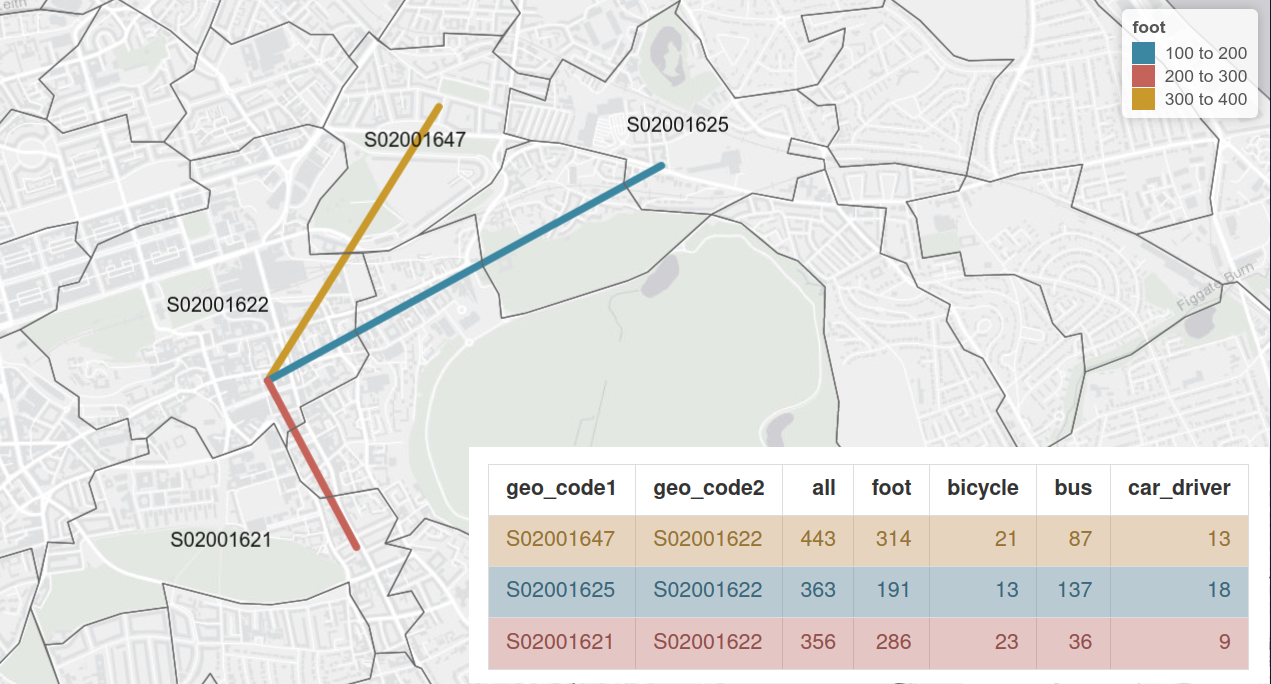
\includegraphics[width=0.8\linewidth]{figures/od-top-3-zones-metafigure} 

}

\caption{Illustration of input data in tabular (bottom right, inset) and geographic form (in the map). Note how the ID codes in the first two columns of the table correspond with IDs in the zone data and how the cells in the 'foot' column are represented geographically on the map.}\label{fig:od}
\end{figure}

The key elements of the jittering approach outlined in this paper are described in the following sub-sections, and are perhaps best understood visually, as illustrated in each of the facetted maps in Figure \ref{fig:jitters}.
The subfigures show the flexibility of approach, with C) and D) demonstrating the use of vertices on the road network as start and end points, building on the observation from spatial network analysis that the density of the transport network is a reasonable proxy for travel demand (Cooper 2018).
Other refinements including weighted subpoints could be used when data sources (e.g.~building footprint areas) are available.

\begin{figure}

{\centering 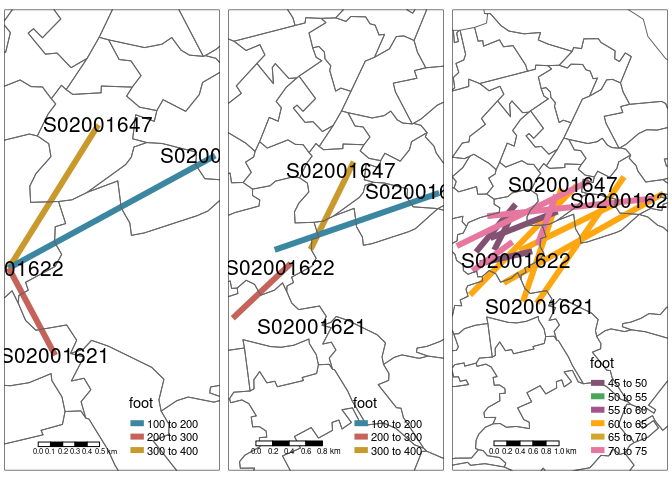
\includegraphics[width=0.8\linewidth]{README_files/figure-latex/jitters-1} 

}

\caption{Illustration of jittering and disaggregation of origin-destination (OD) data with a minimal input dataset. Subfigure A) shows the conventional way of representing OD data as desire lines between zone centroids. Subfigures B) and C) show the same desire lines but with jittered origin and destination locations based on simple random sampling of points and sampling locations on the road network. Subfigure D) shows the combined impact of disaggregation and jittering. Zone limits are represented in grey, while road network is in green.}\label{fig:jitters}
\end{figure}

\hypertarget{sampling-origin-and-destination-points}{%
\subsection{Sampling origin and destination points}\label{sampling-origin-and-destination-points}}

Key to jittering is ensuring that each trip starts and ends in a different place.
To do this, there must be `sub-points' within each zone, one for each trip originating and departing.

The simplest approach is simple random spatial sampling, as illustrated in Figure \ref{fig:jitters} (B), which involves generating random coordinate pairs.
This approach has the advantages of simplicity, requiring no additional datasets, but has the disadvantage that it may lead to unrealistic start and end points, e.g.~with trips being simulated to start in rivers and in uninhabited wilderness areas.

To overcome the limitations of the simple random sampling approach, the universe of possible coordinates from which trips can originate and end can be reduced by providing another geographic input dataset.
This dataset could contain known trip attractors such as city centers and work places, as well as tightly defined residential `subzones.'
For highly disaggregated flows in cases where accurate building datasets are available, building footprints could also be used.
A useful, and widely available (Barrington-Leigh and Millard-Ball 2017), input for subsampling is a transport road network, as illustrated in Figure \ref{fig:jitters} (C).
Additional refinements to the stochastic selection of origin and destination based on weights relating to other datasets are possible, as discussed in the final section.

\hypertarget{disaggregation}{%
\subsection{Disaggregation}\label{disaggregation}}

Both of the jittering techniques outlined above generate more diffuse route networks.
However, a problem with OD datasets is that they are often highly variable: one OD pair could represent 1 trip, while another could represent 1000 trips.
To overcome this problem a process of disaggregation can be used, resulting in additional OD pairs within each pair of zones.
The results of disaggregation are illustrated geographically in Figure \ref{fig:jitters} (D) and in terms of changes to attributes, in Tables \ref{tab:dis1} and \ref{tab:dis2}.
As shown in those tables, updated attributes can be calculated by dividing previous trip counts by the number of OD pairs in the disaggregated representation of the data, 5 in this case.
To determine how many disaggregated OD pairs each original OD pair is split into, a maximum threshold was set: an OD pairs with a total trip count exceeding this threshold (set at 100 in this case) is split into the minimum number of disaggregated OD pairs that reduce the total number of trips below the threshold.

\begin{table}

\caption{\label{tab:dis1}Attribute data associated with an OD pair before disaggregation.}
\centering
\begin{tabular}[t]{lllrr}
\toprule
representation & geo\_code1 & geo\_code2 & all & foot\\
\midrule
original & S02001647 & S02001622 & 443 & 314\\
\bottomrule
\end{tabular}
\end{table}

\begin{table}

\caption{\label{tab:dis2}Attribute data associated with an OD pair after disaggregation.}
\centering
\begin{tabular}[t]{lllrr}
\toprule
representation & geo\_code1 & geo\_code2 & all & foot\\
\midrule
disaggregated & S02001647 & S02001622 & 88.6 & 62.8\\
disaggregated & S02001647 & S02001622 & 88.6 & 62.8\\
disaggregated & S02001647 & S02001622 & 88.6 & 62.8\\
disaggregated & S02001647 & S02001622 & 88.6 & 62.8\\
disaggregated & S02001647 & S02001622 & 88.6 & 62.8\\
\bottomrule
\end{tabular}
\end{table}

\hypertarget{findings}{%
\section{Findings}\label{findings}}

We found that jittering generates desire lines, and route networks, that are more geographically diffuse than those resulting from the established centroid-based approach.
Figure \ref{fig:jittered514} shows the use of simple random sampling and sampling nodes on transport networks with reference to a real world example.
While the simple random sampling method of jittering presented in Figure \ref{fig:jittered514} (B) may be appropriate in some specific cases, we advocate using pre-defined sub-points.
Using sub-points representing vertices on the transport network, as illustrated in Figures \ref{fig:jittered514} C and D, is supported by `spatial network analysis' (SNA) approaches to transport modelling (e.g. Cooper 2018).
Weighted points representing trip origins and destinations such as houses and commercial buildings could also be used.

\begin{figure}

{\centering 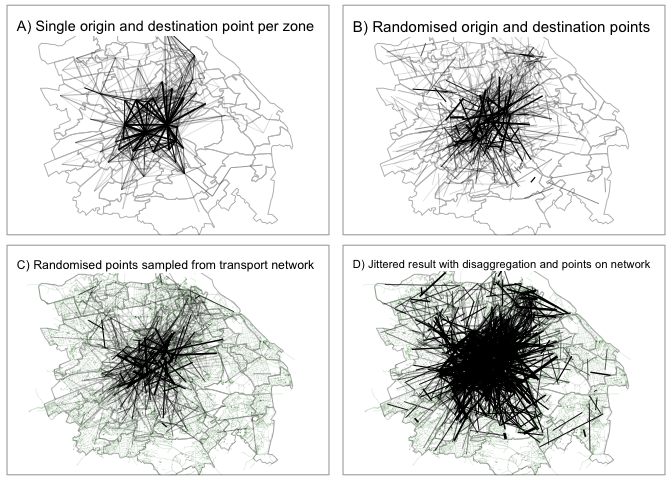
\includegraphics{README_files/figure-latex/jittered514-1} 

}

\caption{Results showing the conversion of OD data to geographic desire lines using population weighted centroids for origins and destinations (A) and jittered results. The jittered results illustrate jittering with simple random sampling of origin and destination locations (B), sampling on the network (C), and sampling on the network plus disaggregation of OD pairs representing more than 100 trips (D).}\label{fig:jittered514}
\end{figure}

The results of converting the desire lines to routes and then route networks are illustrated in Figure \ref{fig:rneted}, which shows progressively more diffuse networks.
Greater disaggregation leads to more diffuse networks as shown in Figure \ref{fig:rneted} (D).

The advantages of this approach include simplicity, low computational cost and flexibility, with disaggregation (and network diffusion) levels adjusted depending on requirements.
Disadvantages relate to the use of random number generators (RNG), which can reduce reproducibility (overcome this by setting a `seed,' which makes the findings reproducible) and influence findings (generate more than one set of results and undertake testing to mitigate this drawback).
Jitting is particularly well suited to modelling walking and cycling, which require diffuse networks.
Taking disaggregation further, the approach can generate one desire line per trip that could feed into agent based models (ABM) such as A/B Street and MATSim (Carlino et al. 2022; Horni, Nagel, and Axhausen 2016).
Jittering has few input data requirements, enabling its use in situations where sub-zones are unavailable.

\begin{figure}

{\centering 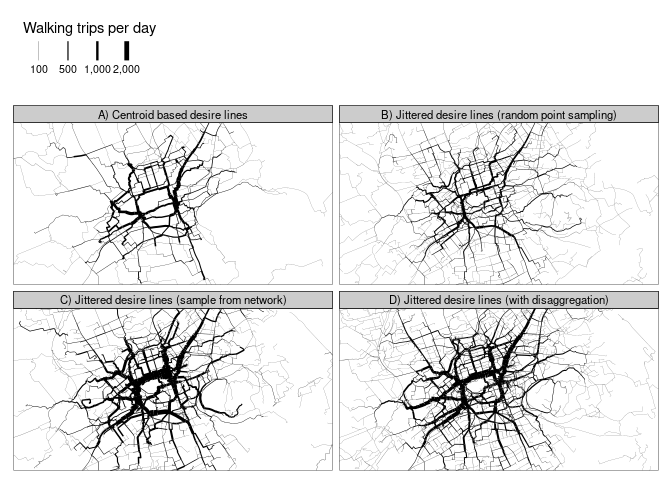
\includegraphics[width=1\linewidth]{README_files/figure-latex/rneted-1} 

}

\caption{Route network results derived from non-jittered OD data (A) and OD data that has been jittered (B to D). The route network results correspond to the desire lines shown in Figure 4, with start and end points sampled from: random locations in geographic space (B); nodes on the transport network network (C); and nodes on the network plus disaggregation of OD pairs representing more than 100 trips (D).}\label{fig:rneted}
\end{figure}

This is, to the best of our knowledge, the first time that stochastic spatial sampling and disagreggation of OD data has been described in a single approach.
The approach is implemented in the open source Rust crate \href{https://github.com/dabreegster/odjitter}{\texttt{odjitter}}.
Implementations in R packages \href{https://itsleeds.github.io/od/}{\texttt{od}} and \href{https://github.com/dabreegster/odjitter/tree/main/r}{\texttt{odjitter}}, an interface to the Rust implementation, enable others to reproduces the findings, raising the possibility of interfaces to other languages.

The results also raise research questions, including:

\begin{itemize}
\tightlist
\item
  Are the jittered results measurably better when compared with counter datasets on the network?
\item
  How would results from jittering OD data compare in other situations, e.g.~to model motor traffic?
\item
  Which jittering settings (including sampling strategies and levels of disaggregation) represent the best `boom for buck' in terms of network accuracy relative to computational requirements?
\item
  And can further refinements, for example sampling with weights to increase the proportion of trips associated with large buildings and commercial centers, or modifying disaggregation threshold values depending on variables such as zone size, improve results?
\end{itemize}

Before further refinements are made, we advocate empirical research to validate the jittering approach outlined in this paper as a foundation for further work on OD data pre-processing and disaggregation.
Such research requires case studies that have both good open OD data and good observed travel behavior data, for example from manual and automatic counters at point locations on the network (Lindsey et al. 2013) and other sources of data such as trajectory datasets from GPS devices (Zheng et al. 2016).

\hypertarget{references}{%
\section*{References}\label{references}}
\addcontentsline{toc}{section}{References}

\hypertarget{refs}{}
\begin{CSLReferences}{1}{0}
\leavevmode\hypertarget{ref-alexander_validation_2015}{}%
Alexander, Lauren, Shan Jiang, Mikel Murga, and Marta C Gonz. 2015. {``Validation of Origin-Destination Trips by Purpose and Time of Day Inferred from Mobile Phone Data.''} \emph{Transportation Research Part B: Methodological}, 1--20. \url{https://doi.org/10.1016/j.trc.2015.02.018}.

\leavevmode\hypertarget{ref-bachir_inferring_2019}{}%
Bachir, Danya, Ghazaleh Khodabandelou, Vincent Gauthier, Mounim El Yacoubi, and Jakob Puchinger. 2019. {``Inferring Dynamic Origin-Destination Flows by Transport Mode Using Mobile Phone Data.''} \emph{Transportation Research Part C: Emerging Technologies} 101: 254--75.

\leavevmode\hypertarget{ref-barrington-leigh_world_2017}{}%
Barrington-Leigh, Christopher, and Adam Millard-Ball. 2017. {``The World's User-Generated Road Map Is More Than 80\% Complete.''} \emph{PLOS ONE} 12 (8): e0180698. \url{https://doi.org/10.1371/journal.pone.0180698}.

\leavevmode\hypertarget{ref-boyce_forecasting_2015}{}%
Boyce, David E., and Huw C. W. L. Williams. 2015. \emph{Forecasting {Urban Travel}: {Past}, {Present} and {Future}}. {Edward Elgar Publishing}.

\leavevmode\hypertarget{ref-buehler_bikeway_2016}{}%
Buehler, Ralph, and Jennifer Dill. 2016. {``Bikeway {Networks}: {A Review} of {Effects} on {Cycling}.''} \emph{Transport Reviews} 36 (1): 9--27. \url{https://doi.org/10.1080/01441647.2015.1069908}.

\leavevmode\hypertarget{ref-abstreet_2022}{}%
Carlino, Dustin, Yuwen Li, Michael Kirk, Mateusz Konieczny, Gedalia Kott, Bruce, Javed Nissar, et al. 2022. \emph{A/{B Street}}. {Zenodo}. \url{https://doi.org/10.5281/zenodo.6331922}.

\leavevmode\hypertarget{ref-cooper_predictive_2018}{}%
Cooper, Crispin H. V. 2018. {``Predictive Spatial Network Analysis for High-Resolution Transport Modeling, Applied to Cyclist Flows, Mode Choice, and Targeting Investment.''} \emph{International Journal of Sustainable Transportation} 0 (0): 1--11. \url{https://doi.org/10.1080/15568318.2018.1432730}.

\leavevmode\hypertarget{ref-friedrich_methods_2009}{}%
Friedrich, Markus, and Manuel Galster. 2009. {``Methods for {Generating Connectors} in {Transport Planning Models}.''} \emph{Transportation Research Record} 2132 (1): 133--42. \url{https://doi.org/10.3141/2132-15}.

\leavevmode\hypertarget{ref-gao_method_2021}{}%
Gao, Hong, Zhenjun Yan, Xu Hu, Zhaoyuan Yu, Wen Luo, Linwang Yuan, and Jiyi Zhang. 2021. {``A {Method} for {Exploring} and {Analyzing Spatiotemporal Patterns} of {Traffic Congestion} in {Expressway Networks Based} on {Origin}--{Destination Data}.''} \emph{ISPRS International Journal of Geo-Information} 10 (5): 288.

\leavevmode\hypertarget{ref-guo_origindestination_2014}{}%
Guo, Diansheng, and Xi Zhu. 2014. {``Origin-{Destination Flow Data Smoothing} and {Mapping}.''} \emph{IEEE Transactions on Visualization and Computer Graphics} 20 (12): 2043--52. \url{https://doi.org/10.1109/TVCG.2014.2346271}.

\leavevmode\hypertarget{ref-he_simple_2018}{}%
He, Biao, Yan Zhang, Yu Chen, and Zhihui Gu. 2018. {``A {Simple Line Clustering Method} for {Spatial Analysis} with {Origin-Destination Data} and {Its Application} to {Bike-Sharing Movement Data}.''} \emph{ISPRS International Journal of Geo-Information} 7 (6): 203. \url{https://doi.org/10.3390/ijgi7060203}.

\leavevmode\hypertarget{ref-horni_multiagent_2016}{}%
Horni, Andreas, Kai Nagel, and Kay W. Axhausen. 2016. \emph{The {Multi-Agent Transport Simulation MATSim}}. {Ubiquity Press}. \url{https://doi.org/10.5334/baw}.

\leavevmode\hypertarget{ref-jafari_investigation_2015}{}%
Jafari, Ehsan, Mason D. Gemar, Natalia Ruiz Juri, and Jennifer Duthie. 2015. {``Investigation of {Centroid Connector Placement} for {Advanced Traffic Assignment Models} with {Added Network Detail}.''} \emph{Transportation Research Record: Journal of the Transportation Research Board} 2498 (June): 19--26. \url{https://doi.org/10.3141/2498-03}.

\leavevmode\hypertarget{ref-katranji_mobility_2016}{}%
Katranji, Mehdi, Etienne Thuillier, Sami Kraiem, Laurent Moalic, and Fouad Hadj Selem. 2016. {``Mobility Data Disaggregation: {A} Transfer Learning Approach.''} In \emph{2016 {IEEE} 19th {International Conference} on {Intelligent Transportation Systems} ({ITSC})}, 1672--77. \url{https://doi.org/10.1109/ITSC.2016.7795783}.

\leavevmode\hypertarget{ref-leurent_stochastic_2011}{}%
Leurent, Fabien, Vincent Benezech, and Mahdi Samadzad. 2011. {``A Stochastic Model of Trip End Disaggregation in Traffic Assignment to a Transportation Network.''} \emph{Procedia - Social and Behavioral Sciences}, The {State} of the {Art} in the {European Quantitative Oriented Transportation} and {Logistics Research} -- 14th {Euro Working Group} on {Transportation} \& 26th {Mini Euro Conference} \& 1st {European Scientific Conference} on {Air Transport}, 20 (January): 485--94. \url{https://doi.org/10.1016/j.sbspro.2011.08.055}.

\leavevmode\hypertarget{ref-li_effects_2019}{}%
Li, Haojie, Yingheng Zhang, Hongliang Ding, and Gang Ren. 2019. {``Effects of Dockless Bike-Sharing Systems on the Usage of the {London Cycle Hire}.''} \emph{Transportation Research Part A: Policy and Practice} 130 (December): 398--411. \url{https://doi.org/10.1016/j.tra.2019.09.050}.

\leavevmode\hypertarget{ref-lindsey_minnesota_2013}{}%
Lindsey, Greg, Steve Hankey, Xize Wang, and Junzhou Chen. 2013. {``The {Minnesota} Bicycle and Pedestrian Counting Initiative: {Methodologies} for Non-Motorized Traffic Monitoring.''} {Minnesota Department of Transportation}. \url{https://www.lrrb.org/media/reports/201324.pdf}.

\leavevmode\hypertarget{ref-liu_snn_2021}{}%
Liu, Qiliang, Jie Yang, Min Deng, Ci Song, and Wenkai Liu. 2021. {``{SNN}\_flow: A Shared Nearest-Neighbor-Based Clustering Method for Inhomogeneous Origin-Destination Flows.''} \emph{International Journal of Geographical Information Science}, 1--27.

\leavevmode\hypertarget{ref-lovelace_propensity_2017}{}%
Lovelace, Robin, Anna Goodman, Rachel Aldred, Nikolai Berkoff, Ali Abbas, and James Woodcock. 2017. {``The {Propensity} to {Cycle Tool}: {An} Open Source Online System for Sustainable Transport Planning.''} \emph{Journal of Transport and Land Use} 10 (1). \url{https://doi.org/10.5198/jtlu.2016.862}.

\leavevmode\hypertarget{ref-martin_origindestination_2018}{}%
Martin, David, Christopher Gale, Samantha Cockings, and Andrew Harfoot. 2018. {``Origin-Destination Geodemographics for Analysis of Travel to Work Flows.''} \emph{Computers, Environment and Urban Systems} 67 (January): 68--79. \url{https://doi.org/10.1016/j.compenvurbsys.2017.09.002}.

\leavevmode\hypertarget{ref-morgan_travel_2020}{}%
Morgan, Malcolm, and Robin Lovelace. 2020. {``Travel Flow Aggregation: Nationally Scalable Methods for Interactive and Online Visualisation of Transport Behaviour at the Road Network Level.''} \emph{Environment \& Planning B: Planning \& Design}, July. \url{https://doi.org/10.1177/2399808320942779}.

\leavevmode\hypertarget{ref-openshaw_optimal_1977}{}%
Openshaw, S. 1977. {``Optimal Zoning Systems for Spatial Interaction Models.''} \emph{Environment and Planning A} 9 (2): 169--84. \url{https://doi.org/10.1068/a090169}.

\leavevmode\hypertarget{ref-opie_commodityspecific_2009}{}%
Opie, Keir, Jakub Rowinski, and Lazar N. Spasovic. 2009. {``Commodity-{Specific Disaggregation} of 2002 {Freight Analysis Framework Data} to {County Level} in {New Jersey}.''} \emph{Transportation Research Record} 2121 (1): 128--34. \url{https://doi.org/10.3141/2121-14}.

\leavevmode\hypertarget{ref-shi_exploring_2019}{}%
Shi, Xiaoying, Fanshun Lv, Dewen Seng, Baixi Xing, and Jing Chen. 2019. {``Exploring the Evolutionary Patterns of Urban Activity Areas Based on Origin-Destination Data.''} \emph{IEEE Access} 7: 20416--31.

\leavevmode\hypertarget{ref-wickham_ggplot2_2016}{}%
Wickham, Hadley. 2016. \emph{Ggplot2: {Elegant Graphics} for {Data Analysis}}. 2nd ed. 2016 edition. {New York, NY}: {Springer}.

\leavevmode\hypertarget{ref-zheng_big_2016}{}%
Zheng, Xinhu, Wei Chen, Pu Wang, Dayong Shen, Songhang Chen, Xiao Wang, Qingpeng Zhang, and Liuqing Yang. 2016. {``Big Data for Social Transportation.''} \emph{IEEE Transactions on Intelligent Transportation Systems} 17 (3): 620--30. \url{http://ieeexplore.ieee.org/abstract/document/7359138/}.

\end{CSLReferences}

\end{document}
